\chapter{Testing \& Evaluation}
\label{chapter6}

The testing process was split in two steps. First, an efficiency evaluation of the package was made to determine the computational time needed for the whole logic to run. Finally, each individual component in the package was separately tested in indoor environments, where such a package could be made use of.

\section{Efficiency Test}

Efficiency was an important attribute to the project since the early planning stage, as the solution was aimed to be used in real-time robotics applications. In this section the timing measurements for each module are presented along with a small discussion about the average execution time and whether the original efficiency target was met.

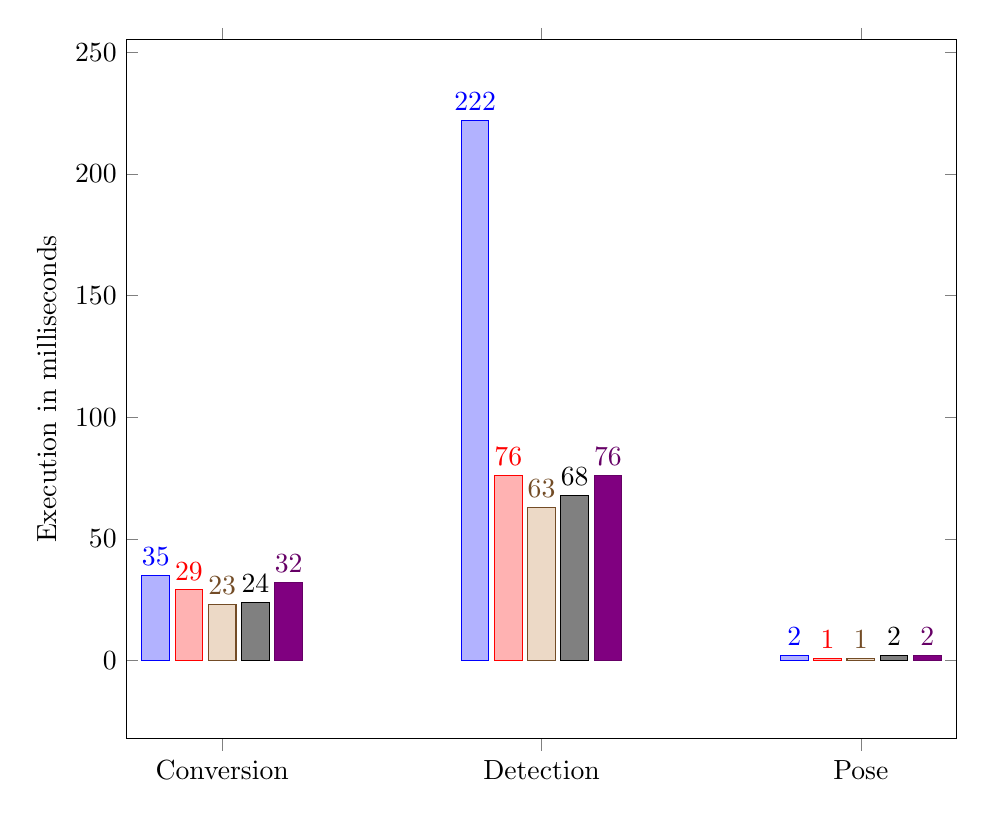
\begin{tikzpicture}
	\begin{axis}[
    	ybar,
        enlargelimits=0.15,
        legend style={at={(0.5,-0.15)},
        anchor=north,legend columns=-1},
        ylabel={Execution in milliseconds},
        symbolic x coords={Conversion, Detection, Pose},
        xtick=data,
        nodes near coords,
        nodes near coords align={vertical},
        width=\textwidth
        ]
        \addplot coordinates {(Conversion, 35) (Detection, 222) (Pose, 2)};
        \addplot coordinates {(Conversion, 29) (Detection, 76) (Pose, 1)};
        \addplot coordinates {(Conversion, 23) (Detection, 63) (Pose, 1)};
        \addplot coordinates {(Conversion, 24) (Detection, 68) (Pose, 2)};
        \addplot coordinates {(Conversion, 32) (Detection, 76) (Pose, 2)};
	\end{axis}
\end{tikzpicture}

From the histogram of the time breakdowns showed above, all of the modules do perform extremely efficiently. In particular, the conversion component takes on average \textbf{28.6 milliseconds} to finish the conversion step. Detecting people on the RGB frame, which is by far the most computationally expensive process, takes an average of only \textbf{101 milliseconds}. Finally, the 3D position estimation module was the fastest one, as it completes the computation in only \textbf{1.6 milliseconds}.

The average computational time needed for the package to carry out the 3D estimation is of only \textbf{43.7 milliseconds}. Therefore, the original objective of developing a ROS package usable in real-time can be considered met.

\section{Module Testing}

In this section the testing is primarily focused on the individual modules. In particular, the detection and pose modules are tested in isolation to check their performance within indoor environments. Note that the conversion module is not tested as it does not have a real impact in the ultimate estimation.

\subsection{Person Detection}

The detection's module tests were carried in two different environments. The robotics lab whose lighting conditions are not the best due to the overexposure and whose space is crammed and cluttered with objects, and the long-room area which offers a sparse area with good lighting conditions. Clutter, occlusions, scale and poor lighting conditions were the situations tested.

\subsubsection{Light conditions, Scale \& Clutter}

\begin{figure}[H]
    \begin{subfigure}{.5\textwidth}
        \centering
        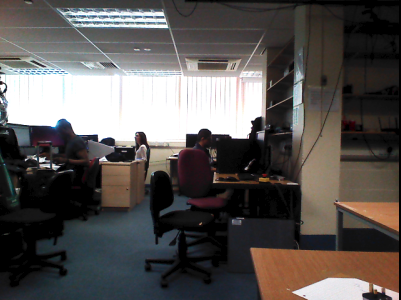
\includegraphics[width=.9\linewidth]{images/chapter6_clutter_light.png}
        \caption{Poor light condition and clutter.}
	\end{subfigure}
    \begin{subfigure}{.5\textwidth}
        \centering
        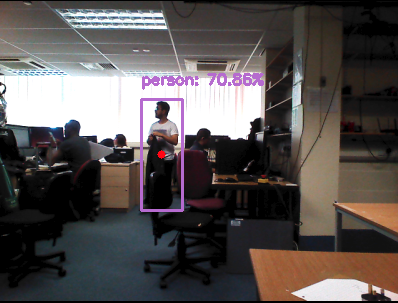
\includegraphics[width=.9\linewidth]{images/chapter6_clutter_light_detection.png}
        \caption{Detection in clutter.}
	\end{subfigure}
    \begin{subfigure}{.5\textwidth}
        \centering
        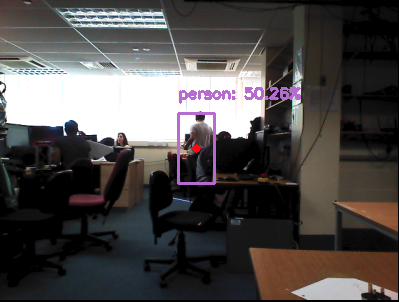
\includegraphics[width=.9\linewidth]{images/chapter6_clutter_light_detection_back.png}
        \caption{Detection in clutter (person showing back).}
	\end{subfigure}
    \begin{subfigure}{.5\textwidth}
        \centering
        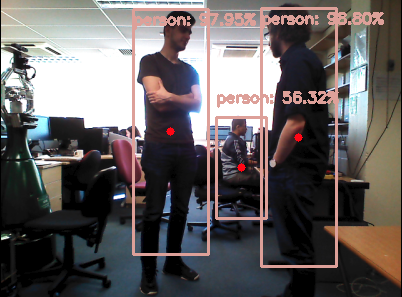
\includegraphics[width=.9\linewidth]{images/chapter6_clutter_standing.png}
        \caption{Multiple detections in clutter.}
	\end{subfigure}
\end{figure}

The outcome of the detection result in poor lighting conditions is variable. In fact, Figure (a) shows a poor performance in the detection result as none of the three subjects in the picture were detected. However, this is not entirely to be attributed to the lighting conditions as the individuals are all partially occluded in the clutter of the lab.

Figure (b) and (c) show an improvement in the detection outcome when one of the individuals is standing in the room. Both situations present difficulties, as in (b) the subject has his lower-body covered by a jacket and in (c) the same person is standing showing only his back while being partially occluded. Which determines the low confidence of 50\% in the detection.

Figure (d) shows a robust detection result when the subjects are standing clearly even in poor lighting conditions and when not facing directly the camera. Moreover, the same figure shows how well the module handles detections at different scales by detecting a third seated person further down the room.

\subsubsection{Occlusions}

\begin{figure}[H]
    \begin{subfigure}{.5\textwidth}
        \centering
        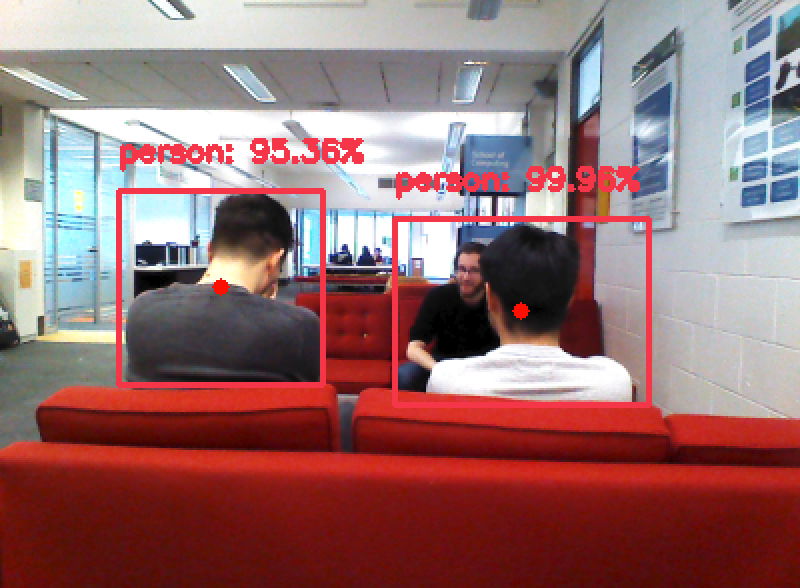
\includegraphics[width=.9\linewidth]{images/chapter6_occlusion_seated.png}
        \caption{Occlusion due to overlapping.}
	\end{subfigure}
    \begin{subfigure}{.5\textwidth}
        \centering
        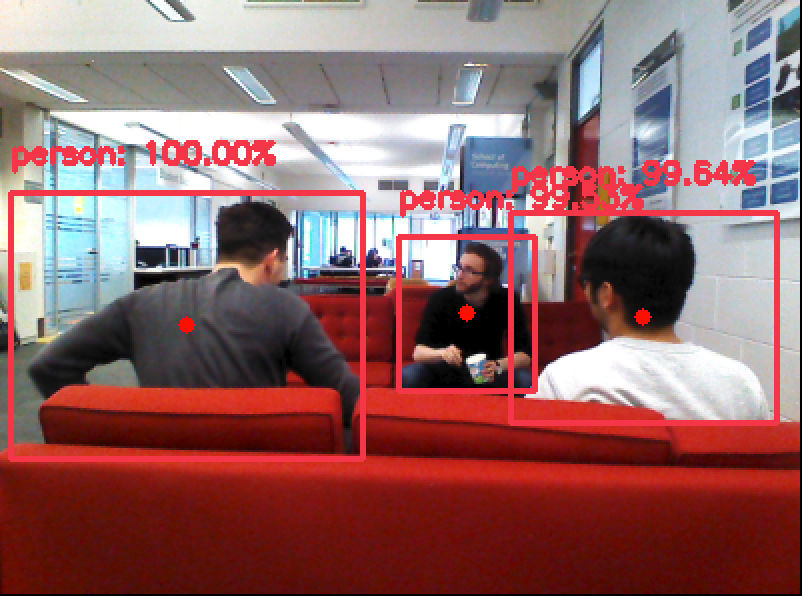
\includegraphics[width=.9\linewidth]{images/chapter6_occlusion_seated_good.png}
        \caption{Correct detection in occlusion.}
	\end{subfigure}
    \begin{subfigure}{.5\textwidth}
        \centering
        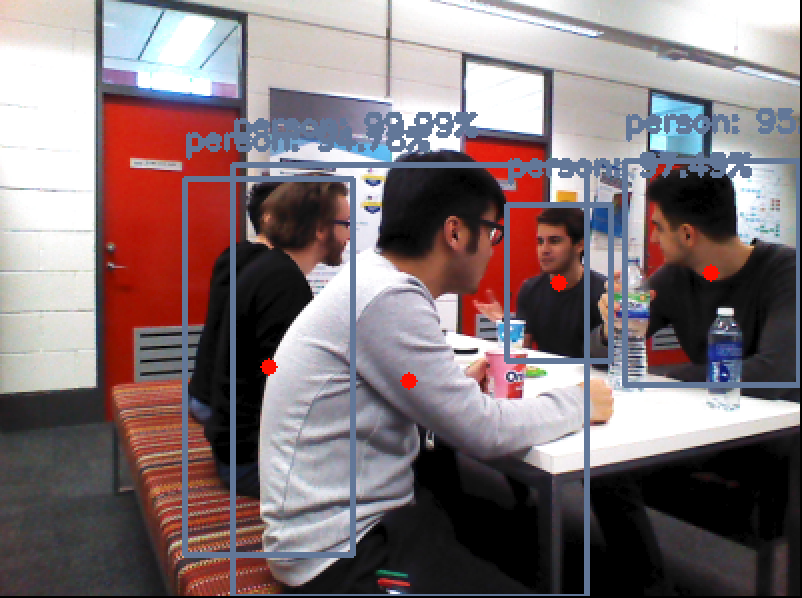
\includegraphics[width=.9\linewidth]{images/chapter6_occlusion_table_back.png}
        \caption{Seated occlusion.}
	\end{subfigure}
    \begin{subfigure}{.5\textwidth}
        \centering
        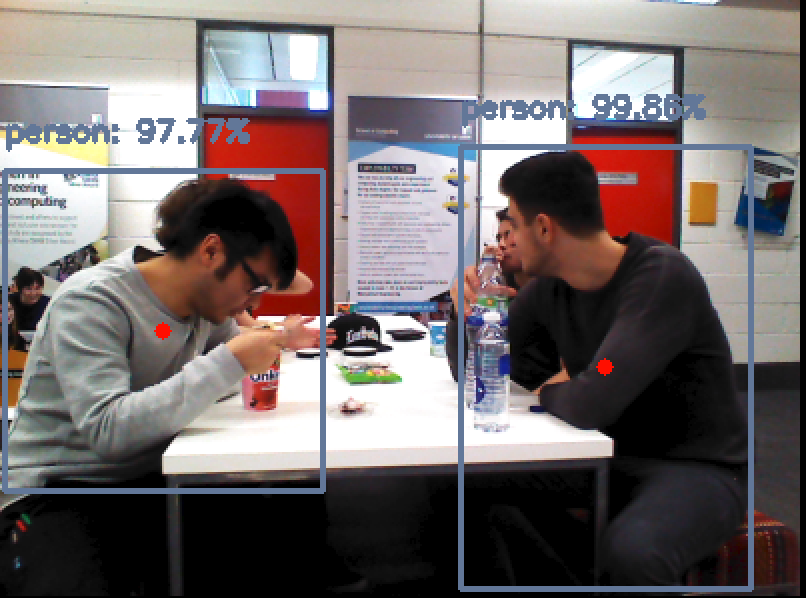
\includegraphics[width=.9\linewidth]{images/chapter6_occlusion_table_side.png}
        \caption{Sideway occlusion.}
	\end{subfigure}
\end{figure}

In Figure (a) the neural network fails at separating between the two subjects sitting to the right of the sofa, although the distinction is clearly visible for a person. Figure (b) shows a good detection result when the occluding person moves to the right. Finally, we notice how in both (a) and (b) the two people sitting with their back towards the camera where detected, even though only a part of their upper-back is showing with an incredible 100\% confidence for one of the subjects in (b).

In Figure (c) the module is able to detect four out of the five participants, in a situation where three of these are either occluded by the table or other subjects. In (d) the same scenario as (c) is presented but from a side perspective. In this occasion only the two people at the for-front are being detected as the remaining three subjects are completely occluded by these.

\subsubsection{Conclusions}

The module can be considered to be highly reliable given its correctness in detecting people in all sorts of positions and variables, as well as its robustness against false positives instances as throughout the testing not once a non-person was detected as such.

\subsection{Pose Estimation}

To test the distance and 3D position computations, three different scenarios were tested out. For each scenario the correct 3D position of each individual was noted down using the point cloud data available in RVIZ. The correct position is then used as a comparison with the estimated one. The red markers in the RVIZ images below show the estimated position while the violet ones the actual one.

\subsubsection{Scenario1}

\begin{figure}[H]
    \begin{subfigure}{.5\textwidth}
        \centering
        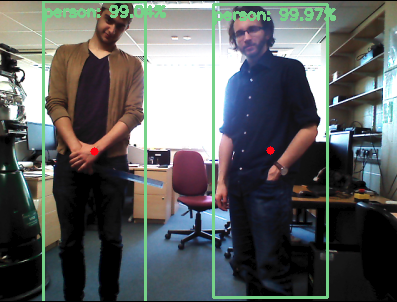
\includegraphics[width=\linewidth]{images/chapter6_scenario1.png}
        \caption{Scenario1 frame.}
        \label{2a}
	\end{subfigure}
    \begin{subfigure}{.5\textwidth}
        \centering
        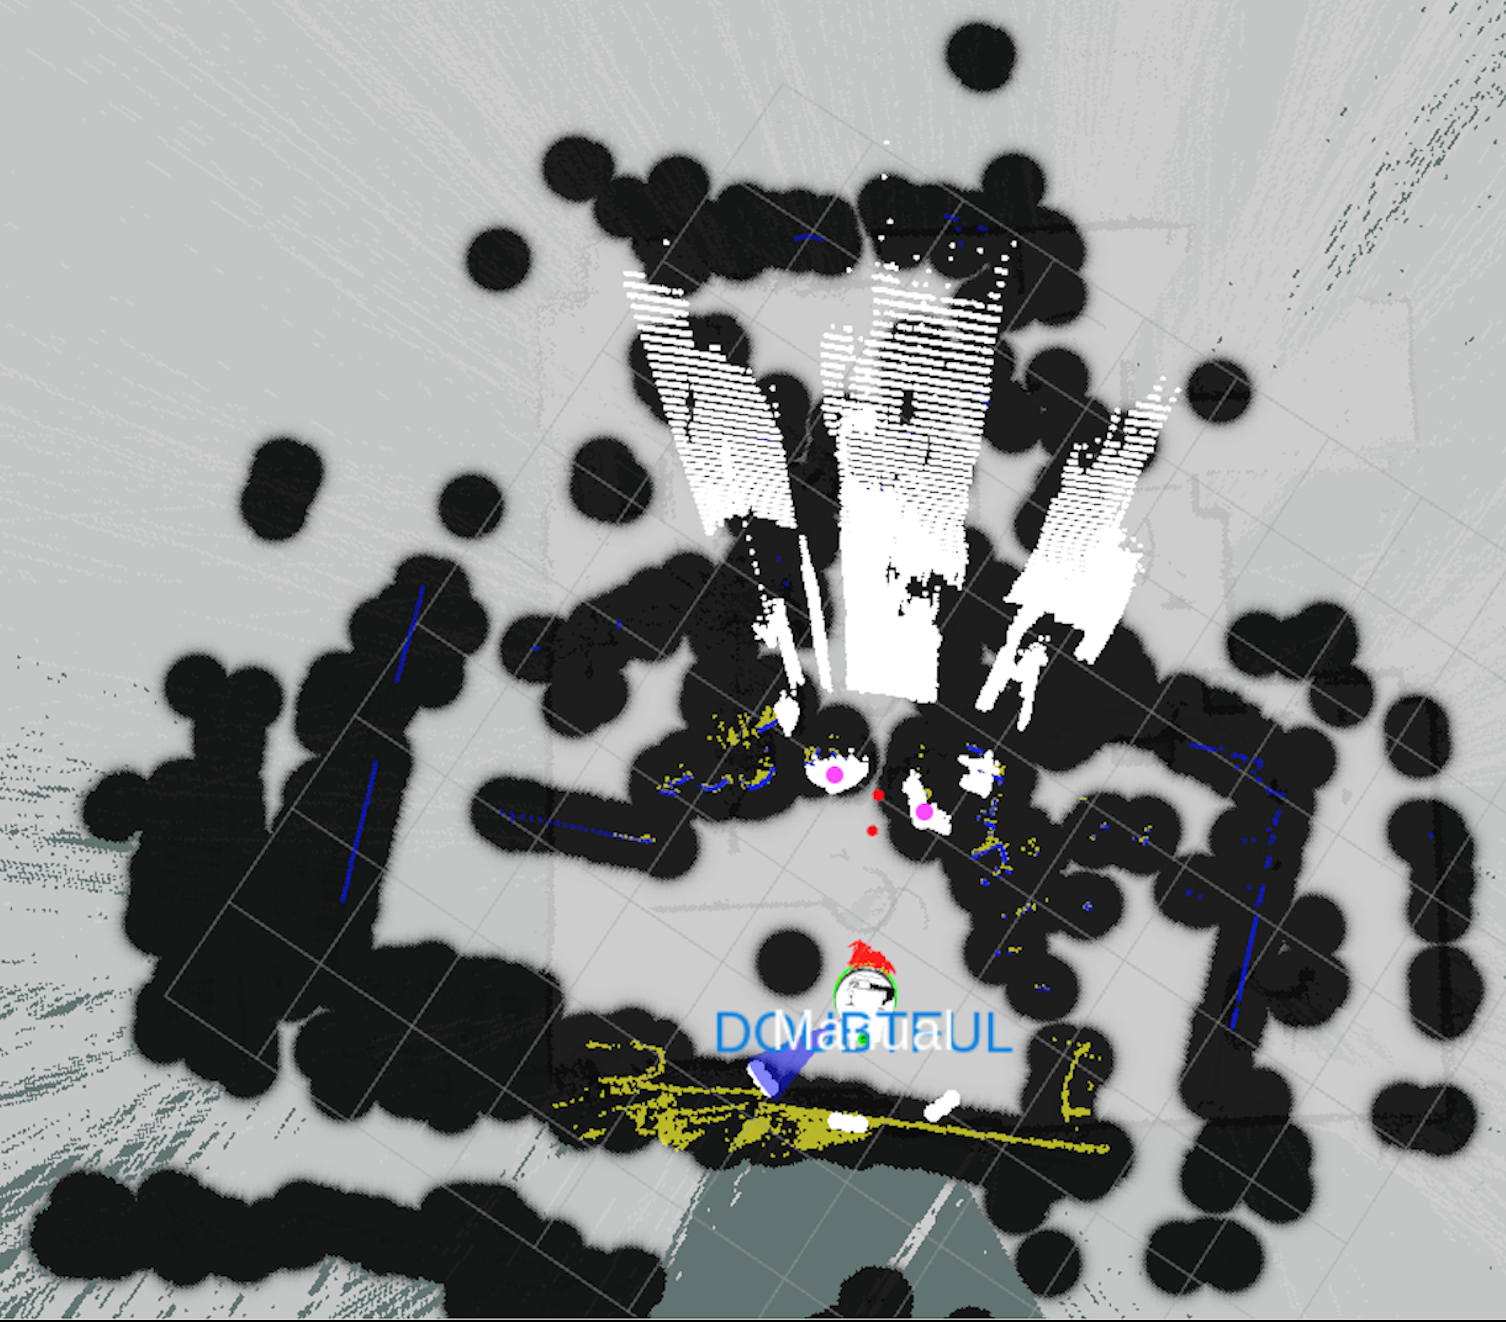
\includegraphics[width=\linewidth]{images/chapter6_rviz_extend.png}
        \caption{Scenario1 markers.}
        \label{2b}
	\end{subfigure}
\end{figure}

\begin{table}[H]
  \centering
  \begin{tabular}{ |p{4cm}|p{2cm}|p{2cm}|p{2cm}|  }
    \hline
    \multicolumn{4}{|c|}{Scenario1: 3D Pose Data} \\
    \hline
    & \textbf{X} & \textbf{Y} & \textbf{Z} \\
    \hline
    Real (Left) & 0.856 & 0.633 & 0.00293 \\
    Estimated (Left) & 0.738 & 0.519 & 0.00203 \\
    Error (Left) & 0.118 & 0.114 & 0.0009 \\
    \hline
    Real (Right) & 0.0497 & 0.264 & 0.00149 \\
    Estimated (Right) & 0.0623 & 0.192 & 0.00475 \\
    Error (Right) & 0.0126 & 0.072 & 0.00326 \\
    \hline
  \end{tabular}
  \label{Scenario1 3D poses.}
\end{table}

The data presented in the above table show for each detection the real and estimated pose as well as the error committed as an absolute error. Figure (b) shows the respective markers representation for the two. The results present a slight error in the 3D pose estimation, although the test subjects are standing close to the robot as shown in Figure (a). Nonetheless, the errors committed are not that big and could still be used for human-robot interaction tasks.

\subsubsection{Scenario2}

\begin{figure}[H]
    \begin{subfigure}{.5\textwidth}
        \centering
        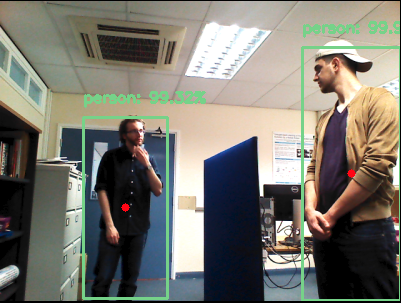
\includegraphics[width=8cm]{images/chapter6_scenario2.png}
        \caption{Scenario2 frame.}
	\end{subfigure}
    \begin{subfigure}{.5\textwidth}
        \centering
        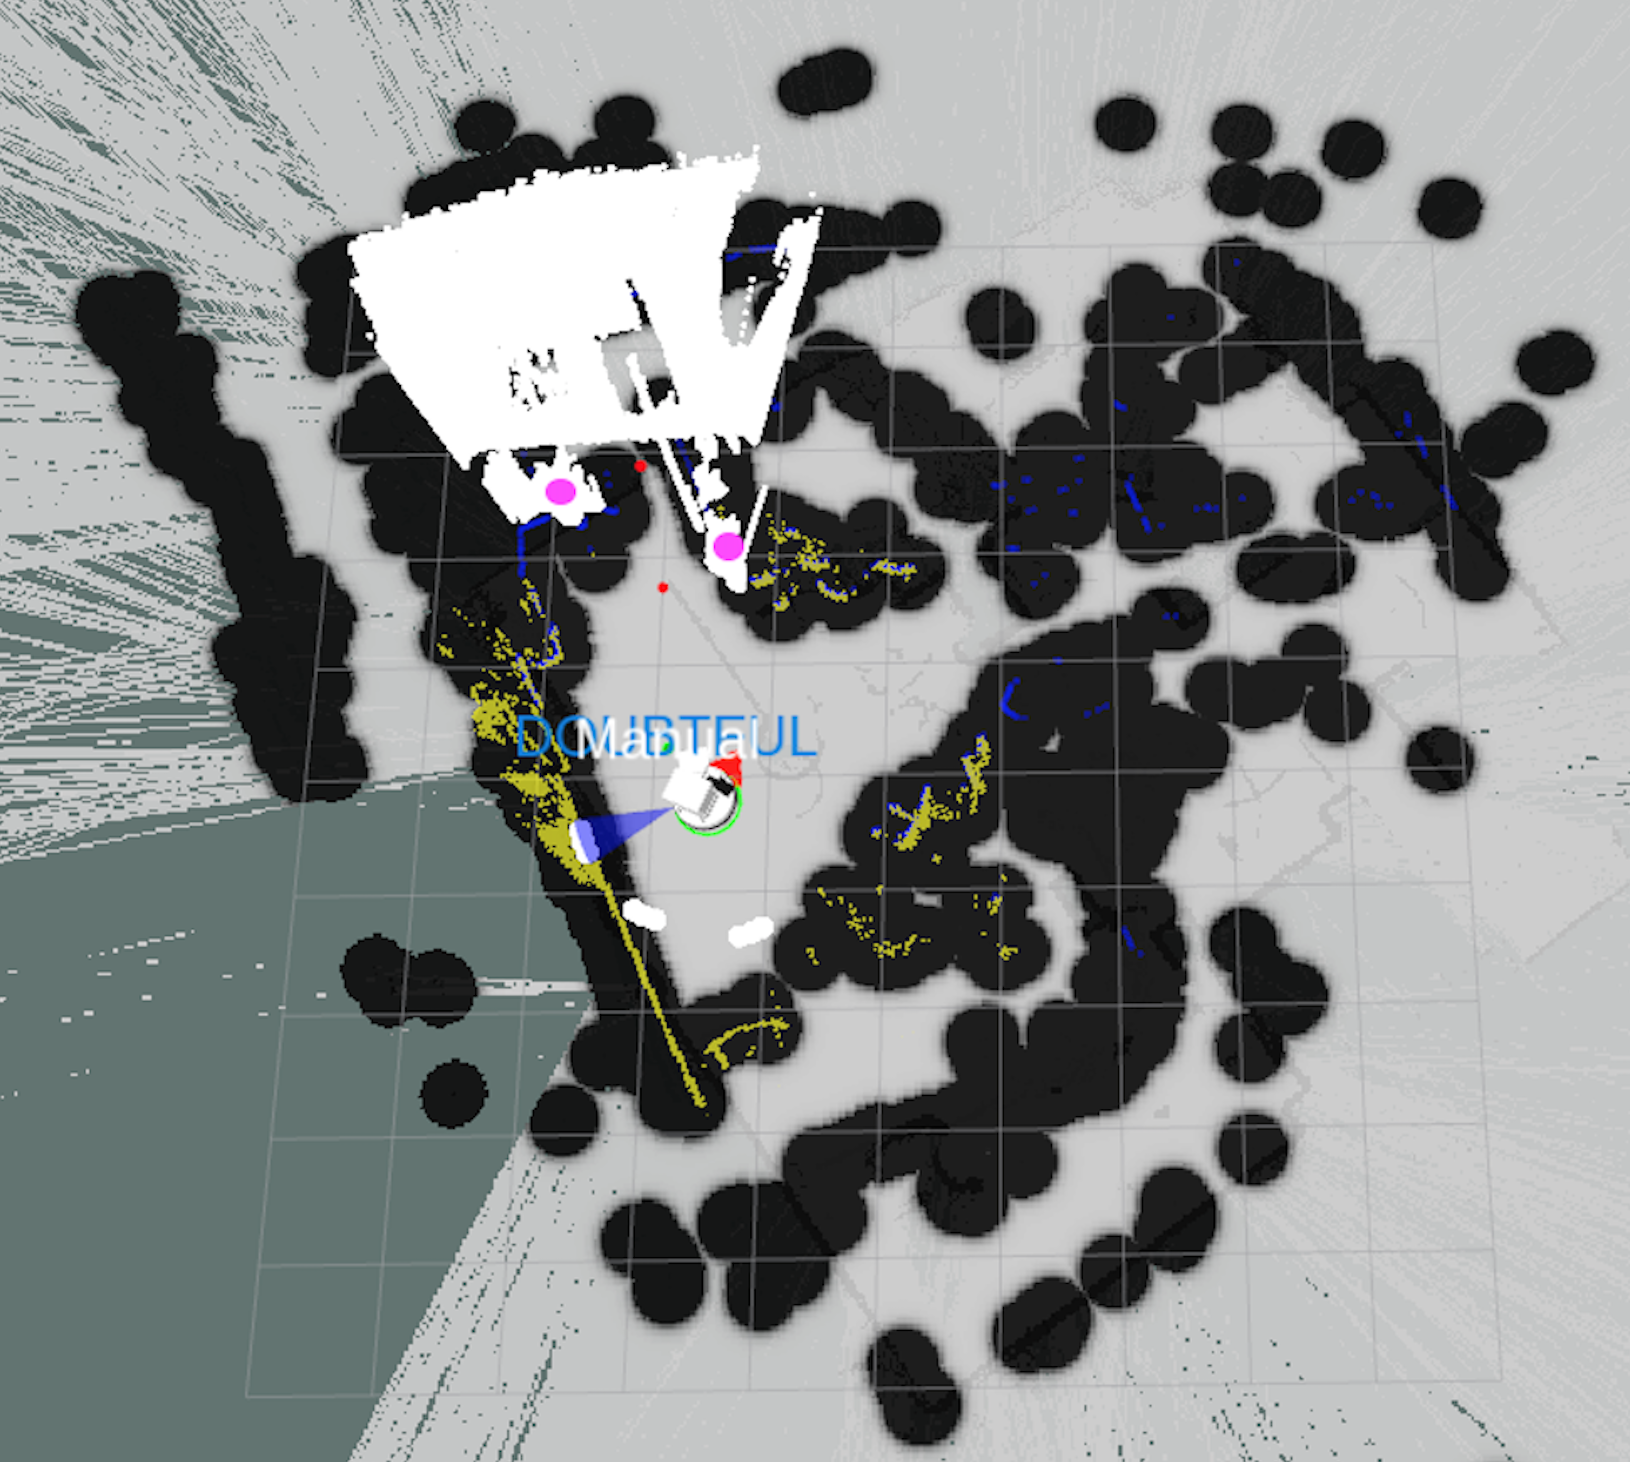
\includegraphics[width=.9\linewidth]{images/chapter6_rviz_extend2.png}
        \caption{Scenario1 markers.}
        \label{2b}
	\end{subfigure}
\end{figure}

\begin{table}[H]
  \centering
  \begin{tabular}{ |p{4cm}|p{2cm}|p{2cm}|p{2cm}|  }
    \hline
    \multicolumn{4}{|c|}{Scenario2: 3D Pose Data} \\
    \hline
    & \textbf{X} & \textbf{Y} & \textbf{Z} \\
    \hline
    Real (Left) & 2.17 & 2.61 & 0.00248 \\
    Estimated (Left) & 2.63 & 2.11 & 0.00357 \\
    Error (Left) & 0.46 & 0.5 & 0.00109 \\
    \hline
    Real (Right) & 1.73 & 1.11 & 0.00547 \\
    Estimated (Right) & 1.4 & 1.67 & 0.00666 \\
    Error (Right) & 0.33 & 0.56 & 0.00119 \\
    \hline
  \end{tabular}
\end{table}

The situation presented in scenario2 is similar to the previous one, with the only difference that the subjects are in different positions and the robot's head is rotated with respect to the base to test the 3D pose transformation process. In fact, the RGB optical frame does not offer a direct transformation link to the map frame, hence intermediate transformations need to take place that include the base link frame.

The results are very similar to scenario1, as the estimations are slightly off to the correct poses with a slight translation in all three coordinates as can be seen in table above and in Figure (b) where the markers are shown.

\subsubsection{Scenario3}

\begin{figure}[H]
    \begin{subfigure}{.5\textwidth}
        \centering
        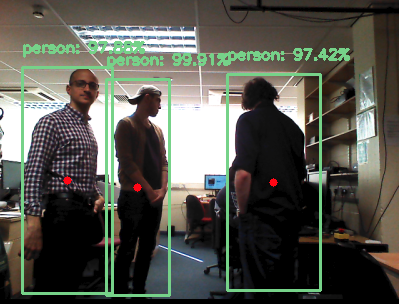
\includegraphics[width=8cm]{images/chapter6_scenario3.png}
        \caption{Scenario1 frame.}
        \label{2a}
	\end{subfigure}
    \begin{subfigure}{.5\textwidth}
        \centering
        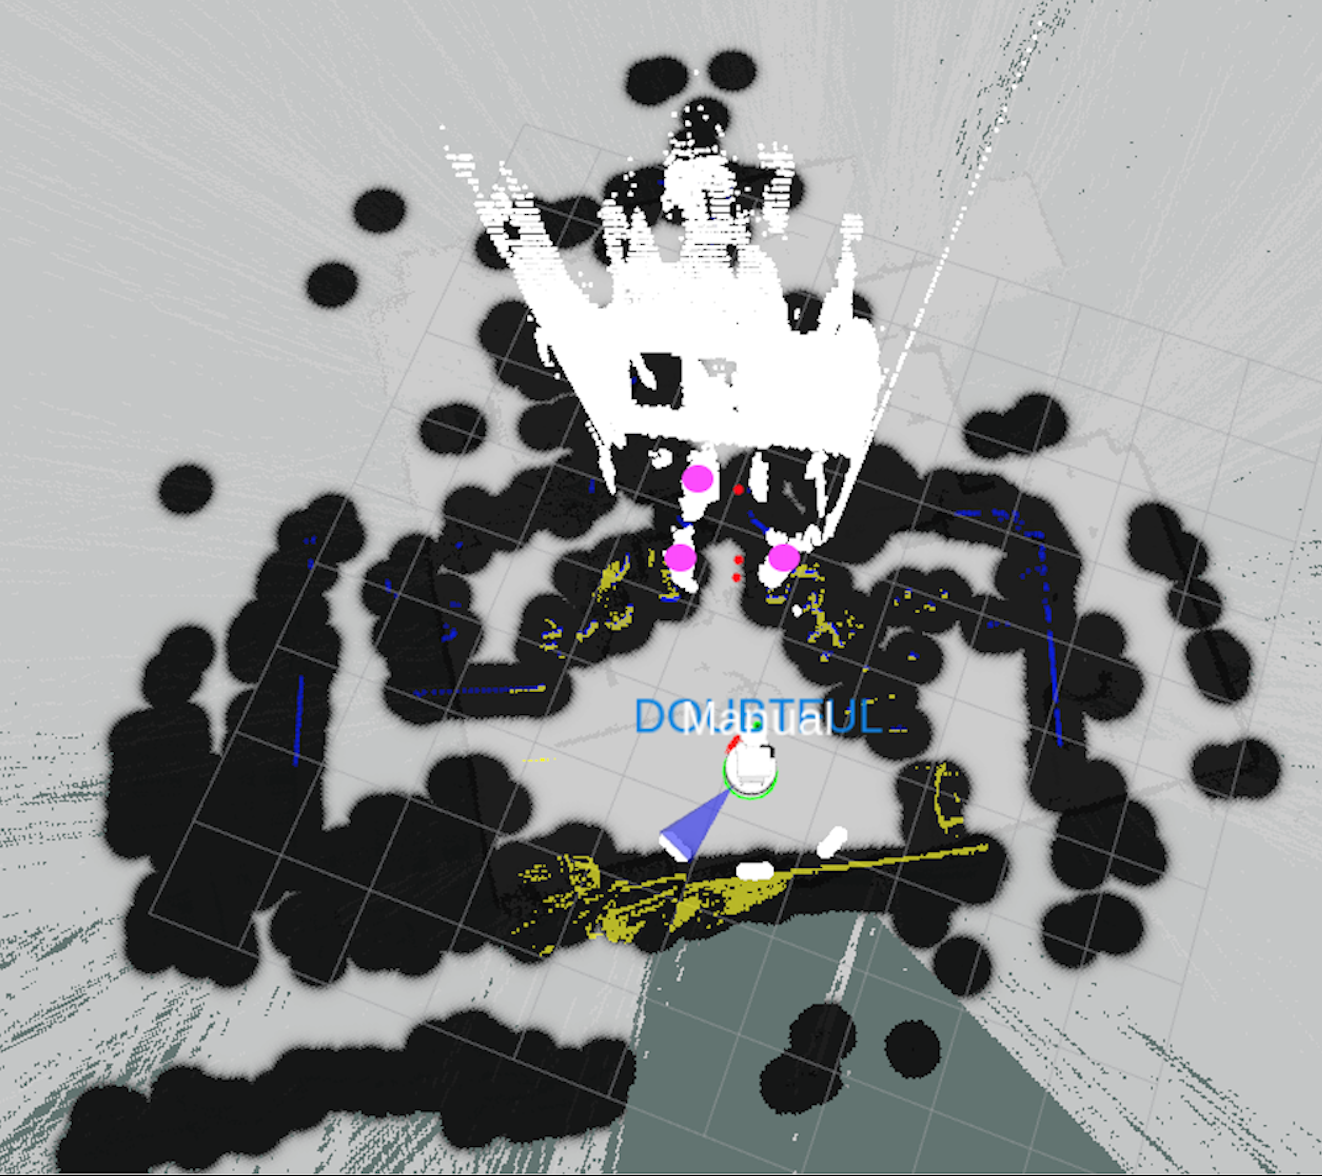
\includegraphics[width=.9\linewidth]{images/chapter6_extend3.png}
        \caption{Scenario1 markers.}
        \label{2b}
	\end{subfigure}
\end{figure}

\begin{table}[H]
  \centering
  \begin{tabular}{ |p{4cm}|p{2cm}|p{2cm}|p{2cm}|  }
    \hline
    \multicolumn{4}{|c|}{Scenario1: 3D Pose Data} \\
    \hline
    & \textbf{X} & \textbf{Y} & \textbf{Z} \\
    \hline
    Real (Left) & 1.33 & 0.0972 & 0.00441 \\
    Estimated (Left) & 1.21 & 0.124 & 0.00203 \\
    Error (Left) & 0.46 & 0.5 & 0.00109 \\
    \hline
    Real (Centre) & 0.0497 & 0.264 & 0.00149 \\
    Estimated (Centre) & 0.283 & 0.344 & 0.00475 \\
    Error (Centre) & 0.2333 & 0.08 & 0.00326 \\
    \hline
    Real(Right) & 1.59 & 0.156 & 0.00456 \\
    Estimated(Right) & 1.37 & 0.271 & 0.00729 \\
    Error (Right) & 0.22 & 0.115 & 0.00273 \\
    \hline
  \end{tabular}
\end{table}

Scenario3 as shown in Figure (a) has three people visible to the camera sensor, whose estimated 3D positions still comprehend small errors, which again makes the estimated poses translate with respect the actual individuals' positions.

\subsubsection{Conclusions}

The distance computation can be considered very robust as in all three test cases the estimation markers were at the same height as the correct poses. However, the same cannot be stated for the 3D conversion phase of the pose module. The translation errors seen, which are of 0.5 metres at most, are probably caused by the the pixel-projection which might suffer from lens distortion, although a distortion correction was applied to the raw image using the distortion matrix which ultimately rectifies the raw colour image. A possible solution to the issue is further discussed in the Evaluation section.
